\chapter{Implementation} \label{chap:implementation}

\section*{}

This chapter describes the details of implementation, in particular the architecture of the tool and the processes involved.

\section{Architecture of the solution} \label{sec:evaluation}
The architecture of this tool was subject of an intense and extensive study and deliberation in order to be implement the best solution.

The best solution would be an architecture that was flexible enough and could be easy to extended,with that the prototype to can achieve more models of assessments and consequently more practices evaluated.

The architecture of the solution can divided into two parts, its database structure and the overall application structure.

\section{Database structure}\label{database}

This model was implemented inside of Scraim, in order to store all the information that is generated an extension of its database was done.

For that purpose several tables in the database were created. Each one one to be flexible enough to store the information of the automatic assessments.

The tables created can be viewed in the Figure \ref{fig:database}, and each purpose is:
\begin{itemize}
	\item \textbf{Model}
	
	This table contains the Models that are stored being classified only for its name, in this case the only model saved is CMMI Level 2.
	\item \textbf{Area}
	
	In this table is stored the Areas, and each Model must have one or more Areas.
	\item \textbf{Goal}
	
	Goals are part of the Area and each Area have one or more Goals.
	\item \textbf{Practice}
	
	Each Practice is a part of a Goal and can be described for its name, summary that gives a simplified description of the practice, its description which is more complete and with some examples in some cases and its weight. Each practice has different weights in the result of the assessment.
	
	\item \textbf{Practice Evaluation}
	
	Represent each Practice evaluation, each practice is evaluated with different criteria and is saved on the database for the presentation of the results.
	
	\item \textbf{Global Assessment}
	
	The Result of the assessment is represent by this table where is saved the global result, which is the aggregation of all practice evaluations for the assessment.
	
\end{itemize}

\begin{figure}[h]
	\begin{center}
		\leavevmode
		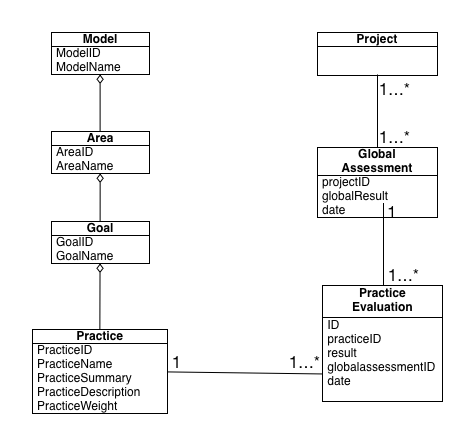
\includegraphics[width=0.8\textwidth]{ClassDiagram}
		\caption{Tables added to database}
		\label{fig:database}
	\end{center}
\end{figure}


On the left side of the Figure \ref{fig:database}, the tables represented are those who are going to be populated with the information from the CMMI for Development and in the right side is where the generated information is going to be stored.

In the Figure \ref{fig:entity-relation} is represented in a systematic way the overall interaction and process in the database, its dependencies and its flow.



\begin{figure}[h]
	\begin{center}
		\leavevmode
		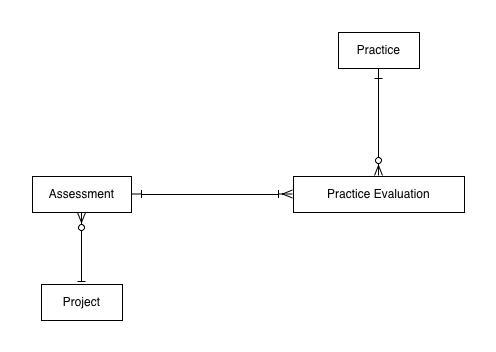
\includegraphics[width=0.6\textwidth]{Entity-Relationship-Model}
		\caption{Entity-relation model}
		\label{fig:entity-relation}
	\end{center}
\end{figure}

With this model of database was possible to achieve the goals and obtain the pretended results.

\section{Module Structure}

As said before, the module structure was object of study and its components were carefully analyzed in order to main a crucial consistency and scalability.

In the Figure \ref{fig:esquema} we can see the overall structure of the module created. The elements shown have a specific role in maintaining the module flexibility. 

\textbf{Database}

Explained in the Section \ref{database}.

\textbf{Abstract Evaluator}

Represents the practices criteria. For each practice the evaluation is different, so will the function that is going to generate the result of that evaluation is different, has a different logic, but has an analog structure. All the Practices Evaluation follow the same structure.
%explicar a estrutura

\textbf{Area Evaluator}
This Part of the Module is a function that depending of the Area, calls all the practice evaluators and receives the result of that.


\textbf{Project Info}
This Function is called to get the project info needed to do the assessment of the assessment of the practice. The info returned will ba passed through the Area Evaluator to the Practice Evaluator represented by the Abstract Evaluator.

\textbf{Main Function}

Its the constructor and main function of the module, calls the functions that evaluate and save the practices evaluations.

\begin{landscape}
\begin{figure}[f]
	\begin{center}
		\leavevmode
		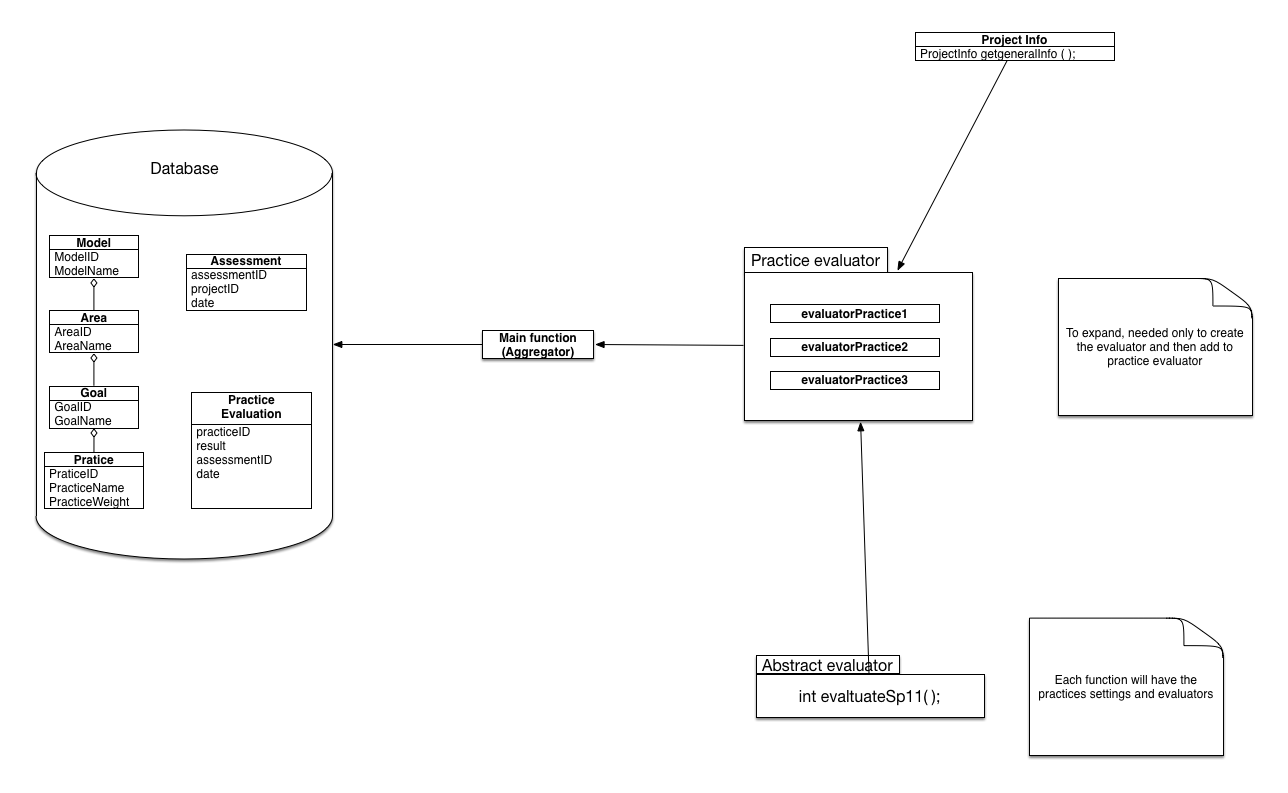
\includegraphics[width=1.5\textwidth]{esquema}
		\caption{Entity-relation model}
		\label{fig:esquema}
	\end{center}
\end{figure}
\end{landscape}

\section{Scalability and Flexibility}

In the Figure \ref{fig:esquema} its observable two notes that describe a way of expanding this model.

The model represented is fully capable of handling expansions of the database and the practices evaluators, the only thing needed is follow some steps:
\begin{itemize}
	\item \textbf{Database Insertion: } Is need to include in the file that starts the database the info of the new models(areas, goals and practices), that are going to be inserted into the tables.
	\item \textbf{Implement all Practices evaluators: } Must be implemented the rules evaluators, those evaluators are represented by the abstract evaluator.
	\item \textbf{Add to the Main Function: } The function that is going to evaluate the practices must be added to the Main Function to be called in the assessment.
\end{itemize}

After this steps the new models added are evaluated and present in the assessment.